\begin{tikzpicture}[>=latex]
    \only<1-2>{
        \node[draw, circle, inner sep = 0, minimum size = 0.7cm] (b) at (3.5, -2) {$\lor$};
        
        \foreach \i in {1, 2, ..., 6}{
            \node[draw, circle, inner sep = 0, minimum size = 0.7cm] (a\i) at (\i, 0) {$\land$};
            \draw[->] (a\i) -- (b);
        }
    }
    \only<3->{
        \node[draw, circle, inner sep = 0, minimum size = 0.7cm] (b) at (4.5, -2) {$\lor$};
        
        \foreach \i in {1, 2, ..., 8}{
            \node[draw, circle, inner sep = 0, minimum size = 0.7cm] (a\i) at (\i, 0) {$\mathds{1}_{C_\i}$};
            \draw[->] (a\i) -- (b);
        }
    }

    \draw[->] (b) -- ++(0, -0.7);
\end{tikzpicture}